\section{Beyond Regularization-Based Approaches}
We have presented the umbrella for categorizing regularization-based approaches. In this section, we move farther and touch the approaches that are beyond purely regularization-based approaches. 

\subsection{Lazy Inference}
Using the KL divergence regularization promotes the online posterior inference one task after one task. However, since the posterior inference in each task is usually not exact, the posterior approximation error might accumulate and grow with seeing more tasks. Specifically, let the function prior be $p(f)$, the exact posterior after $t$ tasks can be represented as $p(f | \data_{1:t})$, and the online inference process is,
\begin{align}
    \underbrace{p(f | \data_{1:t})}_{\text{online posterior}} \propto \underbrace{p(f | \data_{1:t-1})}_{\text{online prior}} \underbrace{p(\data_t | f)}_{\text{likelihood}},
\end{align}
In practice, the posterior inference in each step is not exact, thus we obtain a sequence of distributions $q_0(f), q_1(f), q_2(f), ...$, where  $q_0(f) := p(f)$ and $q_{t}(f) \propto q_{t-1}(f) p(\data_t|f)$. Because the posterior approximation error might accumulate, the knowledge about old tasks will be reduced in each task. After seeing many new tasks, the learner might totally forget the ability learnt from the old tasks. 

To mitigate this problem, \textit{lazy inference} selects and stores a small coreset $\coreset_{t} \subset \data_t$ for each task $t$. One can manipulate the exact posterior to have the expression,
\begin{align}
    p(f | \data^{1:t}) = p(f | \coreset_{1:t}, \data_{1:t} \backslash \coreset_{1:t}) \propto p\left(f | \cup_{t=1}^t (\data_t \backslash \coreset_t)\right) p(\coreset_{1:t} | f),
\end{align}
In the course of online inference, the lazy inference learner approximates the posterior $p\left(f | \cup_{t=1}^t (\data_t \backslash \coreset_t)\right)$. In concrete, the learner obtains a sequence of distributions $\hat{q}_0(f), \hat{q}_1(f), \hat{q}_2(f), ...$, where  $\hat{q}_0(f) := p(f)$ and $\hat{q}_{t}(f) \propto \hat{q}_{t-1}(f) p(\data_{t} \backslash \coreset_{t}|f)$. Finally the true posterior can be approximated as,
\begin{align}
    p(f | \data_{1:t}) \approx q_t(f) \propto \hat{q}_t(f) p(\coreset_{1:t} | f),
\end{align}
Note that $\hat{q}$ is updated by online inference but $q_t$ is obtained directly from $\coreset_{1:t}$. In this way, the coreset mitigates the issue of error accumulation. Since we move the inference of $\coreset_{1:t}$ backwards until the prediction phase, this technique is named \emph{lazy inference}. A visualization of this lazy inference is shown in Figure~\ref{fig:online-inference-1}. We note the lazy inference technique can be applied for both weight-space \citep{nguyen2017variational} and function-space distributional inferences.

\begin{figure}
\centering
%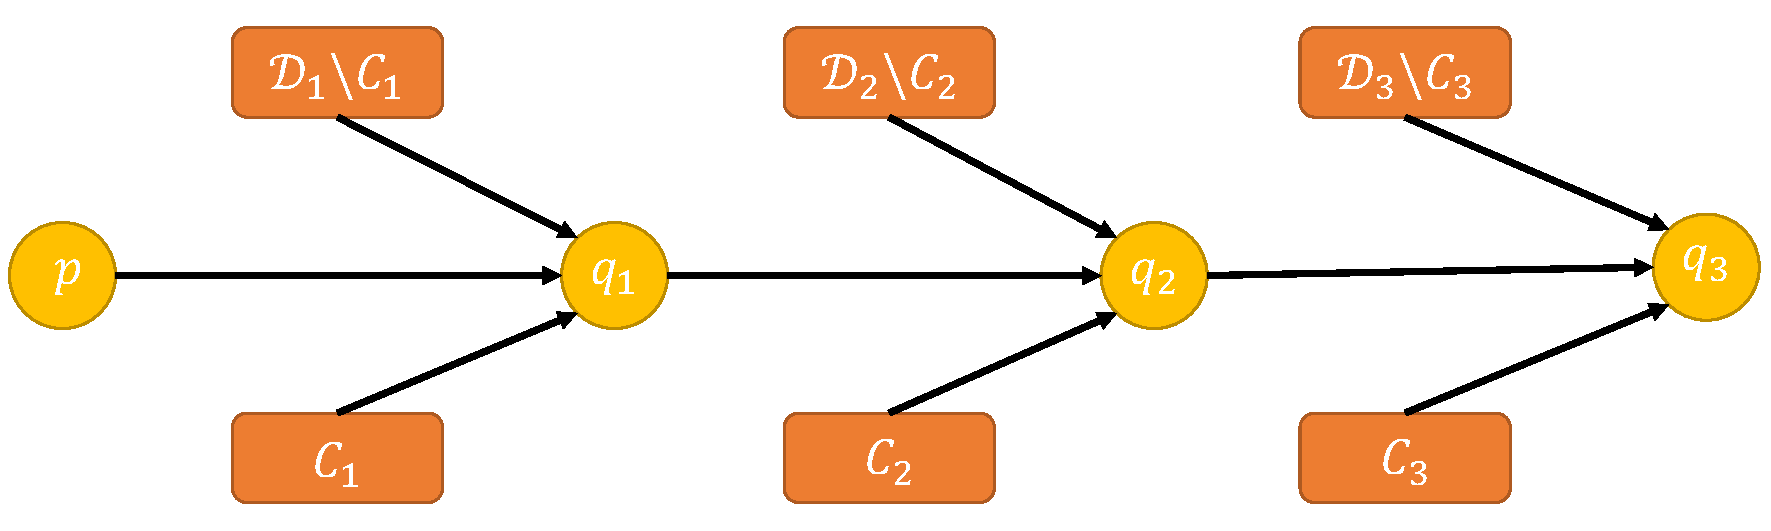
\includegraphics[height=0.16\textwidth]{figures/lazy-inference-1.pdf}
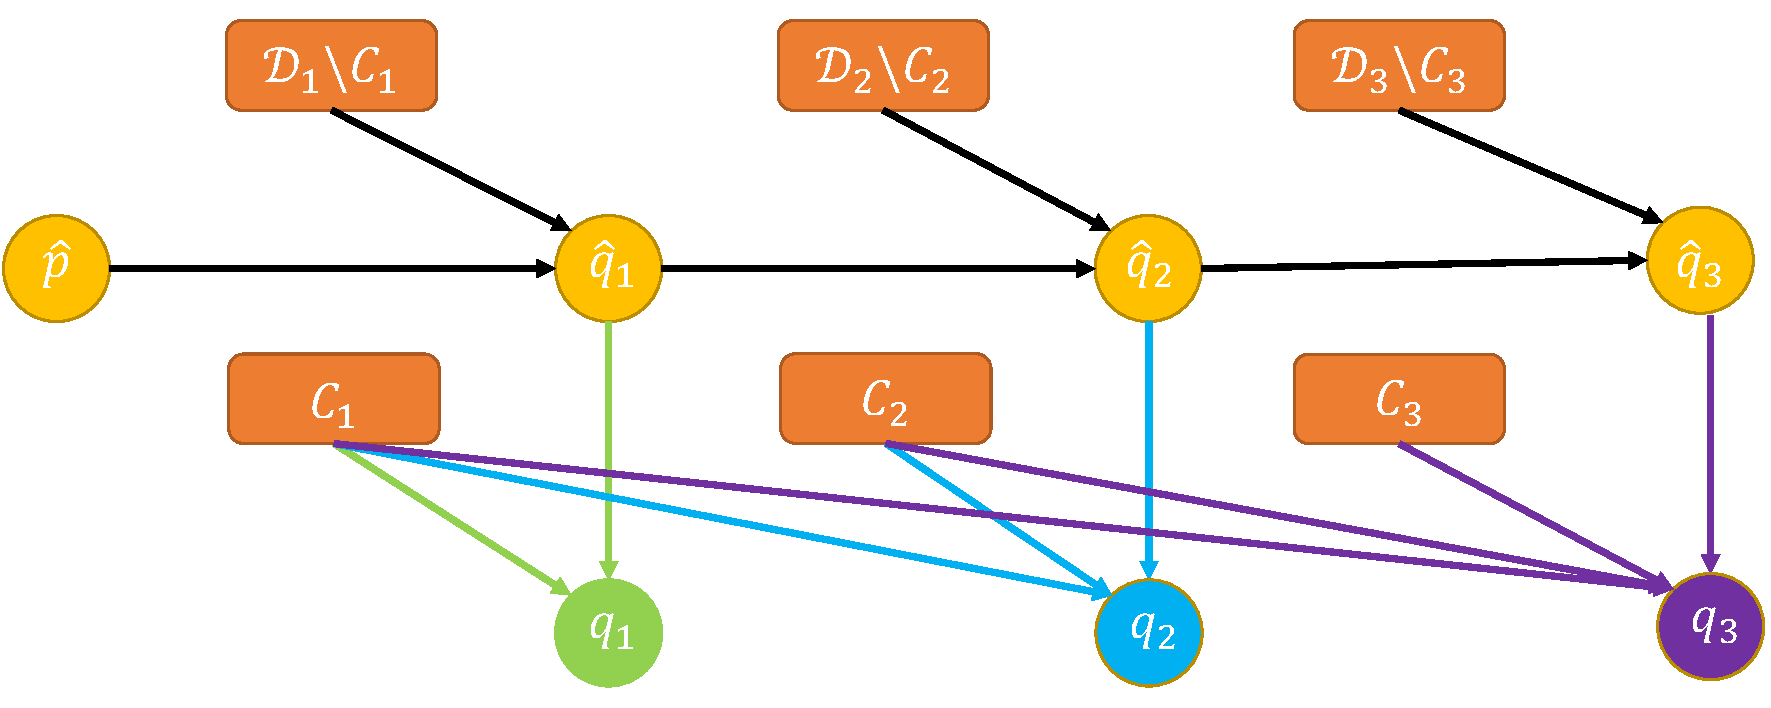
\includegraphics[width=0.9\textwidth]{figures/lazy-inference-2.pdf}
\caption{A visualization of the  the lazy inference, where the coresets $\cup_{i=1}^t \coreset_t$ are left out in the online inference procedure and are incorporated in the prediction procedure.\label{fig:online-inference-1}}
\end{figure}


\subsection{Network Growing}
The catastrophic forgetting problem will not appear if the network is not updated in new tasks, but then it also prevents learning new tasks. To resolve this conflict, progressive networks \citep{rusu2016progressive} propose to grow the network along with seeing new tasks. As shown in Figure~\ref{fig:progress}, given a new task, each layer is expanded with new hidden units and the network only updates the added weights for learning the new task. In this way, progressive networks totally resolve the problem of catastrophic forgetting. Moreover, since the network optimized for old tasks is also used for new tasks, progressive networks enable forward transfer as well. 

However, the network size grows linearly with the number of tasks, which might quickly exceed the memory budget. The progress-and-compress networks \citep{schwarz2018progress} propose to resolve this problem by recursively “compressing” the network into the small subnetwork. In other words, after progressing the network in each task, the overall network is again distilled into the original subnetwork. In this way, the network size keeps constant in the course of continual learning.

\begin{figure}[h]
\centering
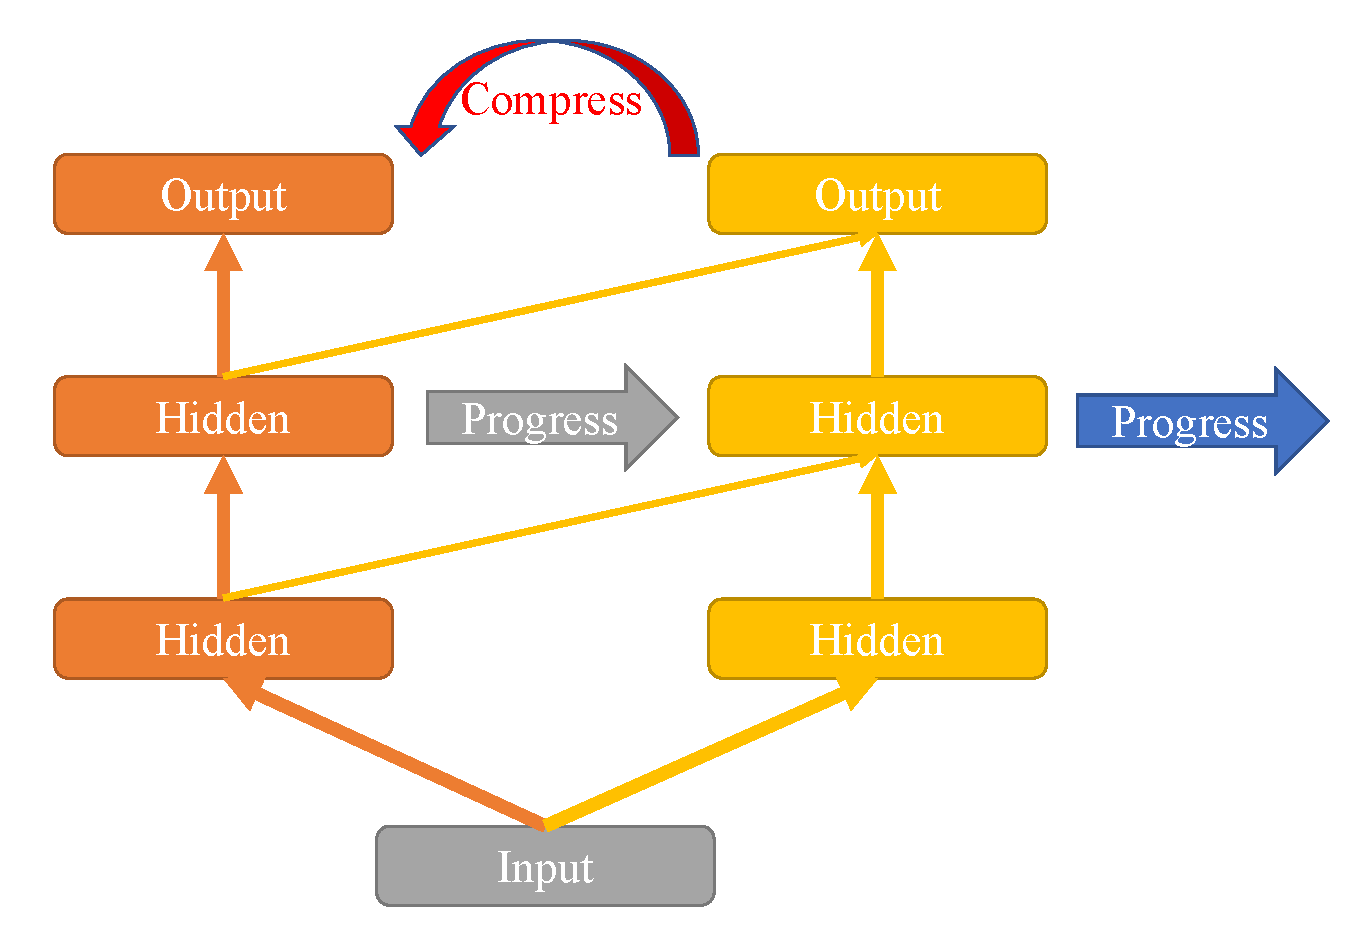
\includegraphics[width=0.6\textwidth]{figures/progressive.pdf}
\caption{The {\color{blue} progressive networks} keep growing the network size, while the {\color{red} progress-and-compress} networks compress the growed network into the original network.  \label{fig:progress}}
\end{figure}

%
%\begin{wrapfigure}[5]{R}{0.3\textwidth}
%    \centering
%    \vspace{-0.6cm}
%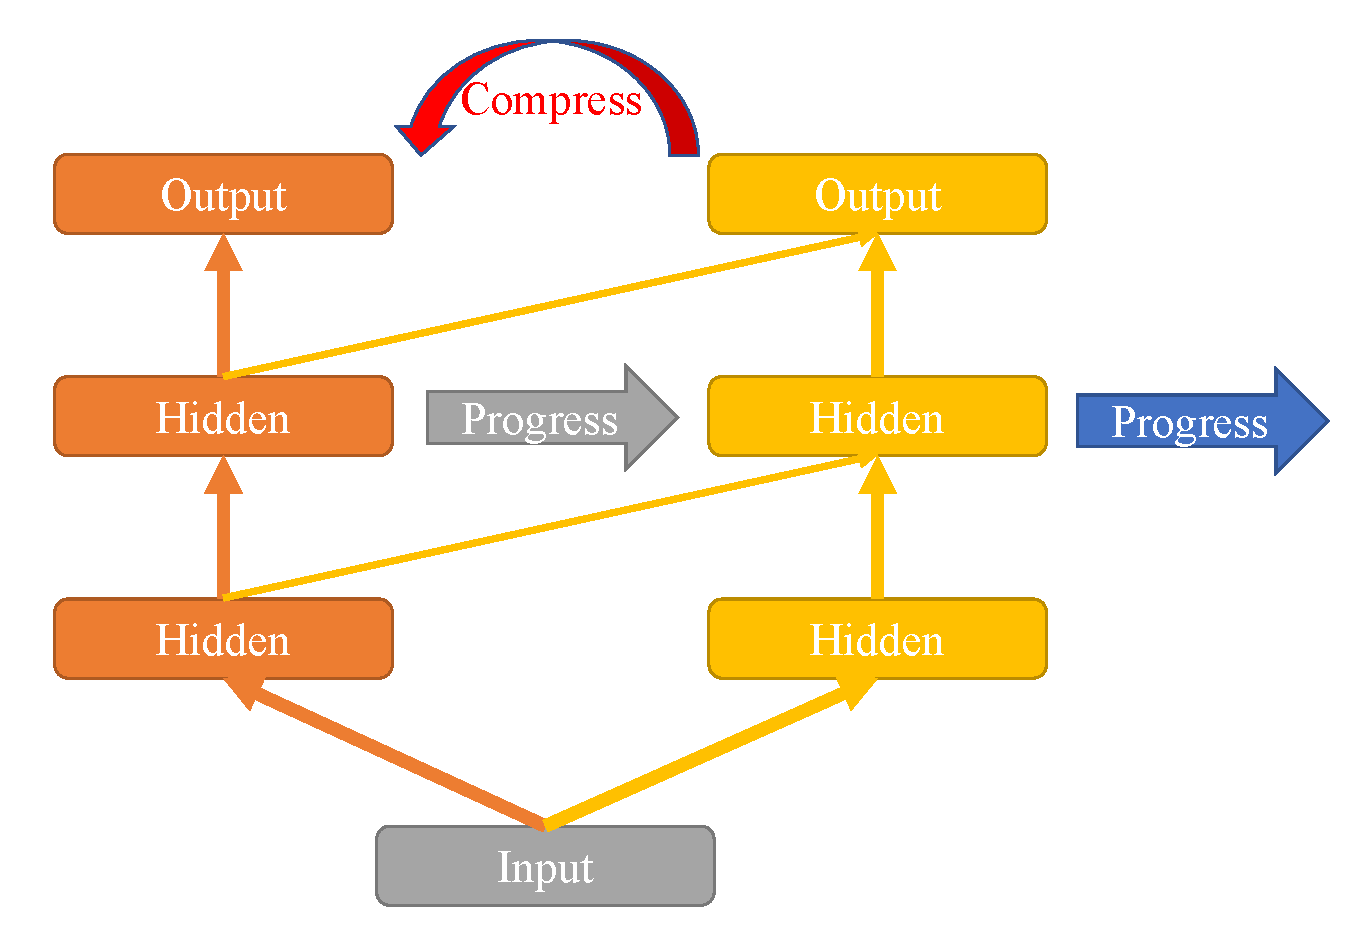
\includegraphics[width=0.5\textwidth]{figures/progressive.pdf}
%\end{wrapfigure}

\subsection{Subspace Methods}

Subspace methods aims at finding a subspace of the network which does not contribute in learning old tasks, thus updating the network in this subspace will not harm previous abilities.

The projection matrix is a common technique to map a vector into an orthogonal subspace. Specifically, let $\bA = [\ba_1, ..., \ba_s] \in \Reals^{d \times s}$ represent the $s$-dimensional subspace within $\Reals^d$. The projection matrix $\bP(\bA) = \bI_d - \bA \left(\bA^{\top}\bA + \alpha \bI_s\right)^{-1} \bA^{\top}$ maps a vector $\bv \in \Reals^{d}$ into the subspace approximately orthogonal to the subspace of $\bA$, where $\alpha$ controls how strongly is the orthogonality. In continual learning, if $\bA^l \in \Reals^{h_{in} \times n}$ consists of all activations of layer $l$ in a neural network for all previous seen inputs, we can then update the weights $\bW^l$ in the direction orthogonal to $\bA^l$. Specifically, let $\delta \bW^l = [\delta \bw_1^l, ..., \delta \bw_{h_{out}}^l] \in \Reals^{ h_{in} \times h_{out}}$ be the original update direction of $\bW^l$, we transform it to $\bP(\bA^l) \delta \bW^l = [\bP(\bA^l) \delta \bw_1^l, ..., \bP(\bA^l) \delta \bw_{h_{out}}^l] $. In consequence, the updated weight will not modify the predictions on previous data points,
\begin{align}
    (\bA^l)^{\top} (\bW^l + \beta \bP(\bA^l) \delta \bW^l) \approx (\bA^l)^{\top} \bW^l,
\end{align}
Although the updates only lie in the subspace of the network, the predictions for the new task still rely on previously learnt weights. Therefore, these approaches still enable forward transfer. Orthogonal Weight Modification (OWM) \citep{zeng2019continual} adopts the projection matrix on activations for continual learning. However, in recurrent neural networks, because the signals will be recursively fed back to the same layer, small perturbations of the weights might cause large changes of the outputs. To further stabilize the forwarding process, \citet{duncker2020organizing} additionally add the projection matrix over the preactivations of each layer.


Instead of attempting to maintain the predictions in each layer, one can directly tackle the whole network. Specifically, a network can be approximated by its linearization, i.e., 
\begin{align}
    f(\bx_i; \bw) \approx \nabla_{\bw_0} f(\bx_i; \bw_0)^{\top}(\bw - \bw_0) + f(\bx_i; \bw_0) ,
\end{align}
Therefore, if we update $\bw$ in the orthogonal subspace of $\nabla_{\bw_0} f(\bx_1; \bw_0), ..., \nabla_{\bw_0} f(\bx_n; \bw_0)$, the predictions of old data points $\bx_1, ..., \bx_n$ will be approximately preserved. Besides the projection matrix, Gram-Schmidt orthogonalization can also be adopted to update in the subspace \citep{farajtabar2020orthogonal}.

Because of the potential structural similarities between tasks, it might even be possible to improve over the old tasks. The Gradient Episodic Memory (GEM) \citep{lopez2017gradient, chaudhry2018efficient}  defines the subspace as,
\begin{align}
    \{g_{\bw} | \innerprod{g_{\bw}}{\nabla_{\bw} \sum_{i=1}^n l(y_i, f(\bx_i; \bw); t_i)} \leq 0\},
\end{align}
Because the direction $g_{\bw}$ is in the similar way with the loss-decreasing direction,  updating along $g_{\bw}$ locally improves the performance over old tasks.

\subsection{Improved Optimizers}
Instead of designing more artful models, one might also achieve continual learning by only improving the optimizer for training the model. \citet{swaroop2019improving} finds that reducing the gradient variances in Variational Continual Learning (VCL) \citep{nguyen2017variational}  vastly improves the performance of VCL. Furthermore, \citet{mirzadeh2020understanding} studies how the flatness of the local minimum is related to the robustness of the model and the performance of continual learning. Empirically they demonstrate that carefully tuning the learning rate schedule and the batch size might provide a large performance boost in continual learning. 

Designing good preconditioners for the gradient update might also help in continual learning. For example, the EWC adds a quadratic regularization $\frac{1}{2}(\bw-\bw_0)\bG (\bw-\bw_0)$ to the fitting loss. By seeing this as a \emph{proximal method}, it leads to using $\bG$ as a preconditioner for the gradient update. Because $\bG$ is the Fisher information matrix, using it as the preconditioner coincides with the \emph{natural gradient optimizer}, which actually achieves the Fisher efficiency in various scenarios \citep{amari1998natural}.  

%\subsection{Meta-Learning}



%\subsection{Coresets in Continual Learning}
%Because storing all previous datasets is intractable, a small subset of examplers, i.e., the coreset, is usually stored for approximating the whole dataset performance. Coresets have become an important technique in many CL approaches. In this subsection, we introduce several representative examples of how to take advantage of the coresets.
%
%Specifically, we let $\bZ = \{\bz_i^0\}_{i=1}^m \in \xdomain^m$ be the coreset to be representative of previous data points. The most straighforward approach is to use $\bZ$ in the function space distance,
%\begin{align}
%   \text{Z-FSD: } \frac{n_0}{m}\sum_{i=1}^{m} \frac{1}{2}\left(f\left(\bz^0_i; \bw\right) - f\left(\bz^0_i; \bw_0\right)\right)^2,
%\end{align}
%Similarly, we can use the coreset $\bZ$ to approximate the mean term in the function-space KL,
%\begin{align}
%    \text{Z-KL-FSD: }  \frac{1}{2} (f(\bZ^0; \bw) - f(\bZ^0; \bw_0))^{\top} \bK_0(\bZ^0, \bZ^0)^{-1} (f(\bZ^0; \bw) - f(\bZ^0; \bw_0)),
%\end{align}
%Furthermore, instead of simply replacing $\bX^0$ with $\bZ^0$, we can consider a more careful design to use $\bZ^0$ for approximation. Note that   linearizing the network derives the GP prior $f(\bx; \bw) \sim \GP(f(\cdot; \bw_0), k_0)$, thus we can adopt the Nystrom approximation from the GP to approximate $f(\bx; \bw)$,
%\begin{align}
%    f(\bx; \bw) \approx \hat{f}(\bx; \bw) \defas f(\bx; \bw_0) + k_0(\bx, \bZ^0) \bK_0(\bZ^0, \bZ^0)^{-1} \left(f(\bZ^0; \bw) - f(\bZ^0; \bw_0)\right),
%\end{align}
%Plugging $\hat{f}(\bx; \bw)$ into the function space distances, we obtain the Nystrom approximated function space distances,
%\begin{align}
%     \text{N-Z-FSD: } &\frac{1}{2}\|\hat{f}(\bX^0; \bw) - f(\bX^0; \bw_0)\|_2^2
%     \notag \\
%     =&\frac{1}{2} df(\bZ^0; \bw)^{\top} \bK_0(\bZ^0, \bZ^0)^{-1} \bK_0(\bZ^0, \bX^0)\bK_0(\bX^0, \bZ^0) \bK_0(\bZ^0, \bZ^0)^{-1} df(\bZ^0; \bw),
%\end{align}
%where we define $df(\bZ^0; \bw) := f(\bZ^0; \bw) - f(\bZ^0; \bw_0)$. Moreover, we can plug $\hat{f}$ into the KL-FSD, 
%\begin{align}
%    \text{N-Z-KL-FSD: } 
%    &\frac{1}{2}df(\bZ^0; \bw)^{\top} \bK_0(\bZ^0, \bZ^0)^{-1} \bK_0(\bZ^0, \bX^0) \bK_0(\bX^0, \bX^0)^{-1} \bK_0(\bX^0, \bZ^0) \bK_0(\bZ^0, \bZ^0)^{-1} df(\bZ^0; \bw) \notag \\
%    &= \frac{1}{2}df(\bZ^0; \bw)^{\top} \bK_0(\bZ^0, \bZ^0)^{-1}df(\bZ^0; \bw),
%\end{align}
%where we used the equality $\bK_0(\bZ^0, \bX^0) \bK_0(\bX^0, \bX^0)^{-1} \bK_0(\bX^0, \bZ^0) = \bK_0(\bZ^0, \bZ^0)$, when $\bZ^0 \subset \bX^0$. Interestingly we observe that N-Z-KL-FSD is the same as Z-KL-FSD.
%
